‫\فصل{سند الویت‌بندی ریسک‌ها}
‫
‫برای اولویت‌بندی ریسک‌های موجود، باید به احتمال وقوع و شدت عواقب هر یک در صورت وقوع توجه کرد. از این رو نمودار نقطه‌های ریسک‌ها را برحسب این دو معیار رسم می‌کنیم. لازم به ذکر است که در نمودار هر چقدر به سمت گوشه راست بالا برویم، ریسک با الویت بالاتری داریم.
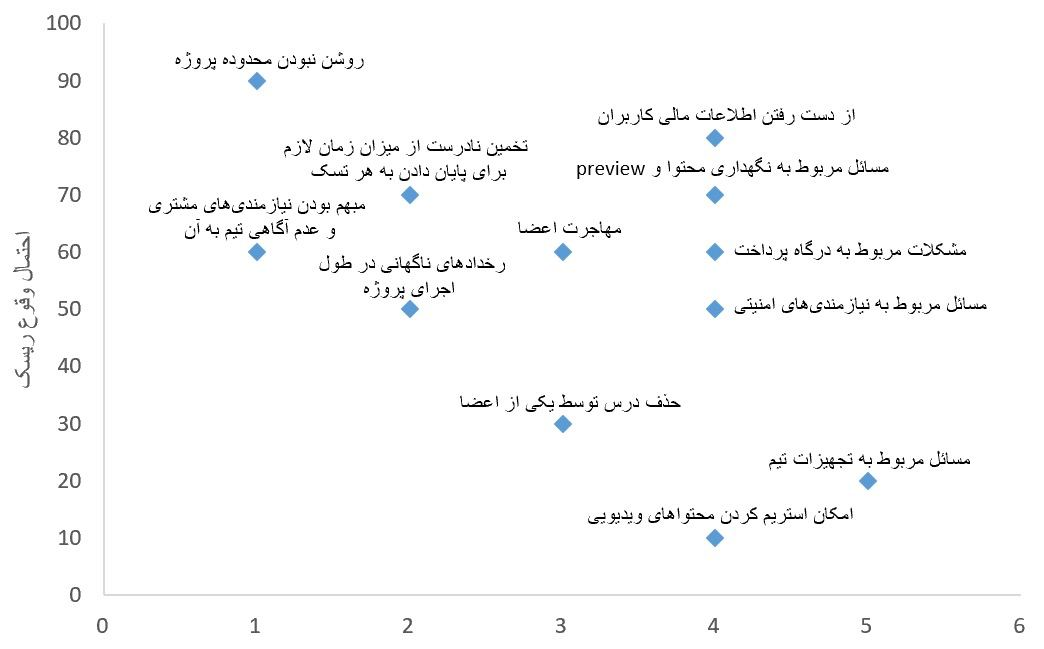
\includegraphics[scale=0.4]{figs/risks_prioritize.jpeg}

‫از این رو اولویت ریسک‌ها به ترتیب زیر است:
‫\شروع{شمارش}
‫\فقره روشن نبودن محدوده پروژه 
‫\فقره از دست رفتن اطلاعات مالی کاربران
‫\فقره مسائل مربوط به نگهداری محتوا و preview
‫\فقره تخمین‌ نادرست از میزان زمان لازم برای پایان دادن به هر تسک
‫\فقره مشکلات مربوط به درگاه پرداخت
‫\فقره مهاجرت اعضا
‫\فقره مبهم بودن نیازمندی‌های مشتری و عدم آگاهی تیم به آن
‫\فقره مسائل مربوط به نیازمندی‌های امنیتی
‫\فقره رخدادهای ناگهانی در طول اجرای پروژه
‫\فقره حذف درس توسط یکی از اعضا
‫\فقره مسائل مربوط به تجهیزات تیم
‫\فقره امکان استریم کردن محتواهای ویدیویی
‫
‫\پایان{شمارش}